\documentclass{article}
\usepackage{graphicx}

\begin{document}
\title{Mirai botnet}
\author{Abhinav Narain}
\maketitle

\section{Mirai Activity and Results}
\subsection{Testbed Setup}
The setup was first made in Virtual environment and then ported to
actual machines on a private network in lab.
\begin{itemize}
\item Linux Box DNS server 
\item Linux Box CNC server
\item Linux Box or Raspberry Pi - client 
\end{itemize}
Figure~\ref{fig:setup} shows the testbed setup on the wireless network.

\subsection{Breakdown of Mirai Bot(client) Activity}
The following steps are performed by Mirai bot.
\begin{enumerate}
\item Sets up some certain data structures, and kills a previous
  instance is running
\item Connects to CNC server after resolving the IP address using a
  DNS packet to DNS server  
\item executes a \textit{fork()} system call to do a SYN scan for a range of IP addresses by
  transmitting TCP SYN frames using RAW sockets  
\item Run an infinite loop waiting for SYN responses for further
  conducting a programmed TELNET login sequence  
\item Wait for attacks from a CNC server and executes a \textit{fork()} system call to launch
  an attack for a period of time -- one of which is a UDP flood attack
  conducted for 5 seconds~\ref{fig:mirai_cnc_server}. Following which the child process kills
  it's parent process (and thereby killing itself) and hence the attack is stopped.
\end{enumerate}

\subsection{Expected Output of EMI}

\begin{itemize}
\item  Step 2 above should produce an EMI on spectrogram corresponding
  to SYN packets transmitted in bulk to certain subnets.  
\item  Step 4 should show EMI on spectrogram corresponding to UDP
  flooding  
\end{itemize}
\subsection{Spectrogram of Lenovo Laptop}
Experiments conducted by running Mirai bot on Lenovo laptop.
\begin{figure}[h]
\centering
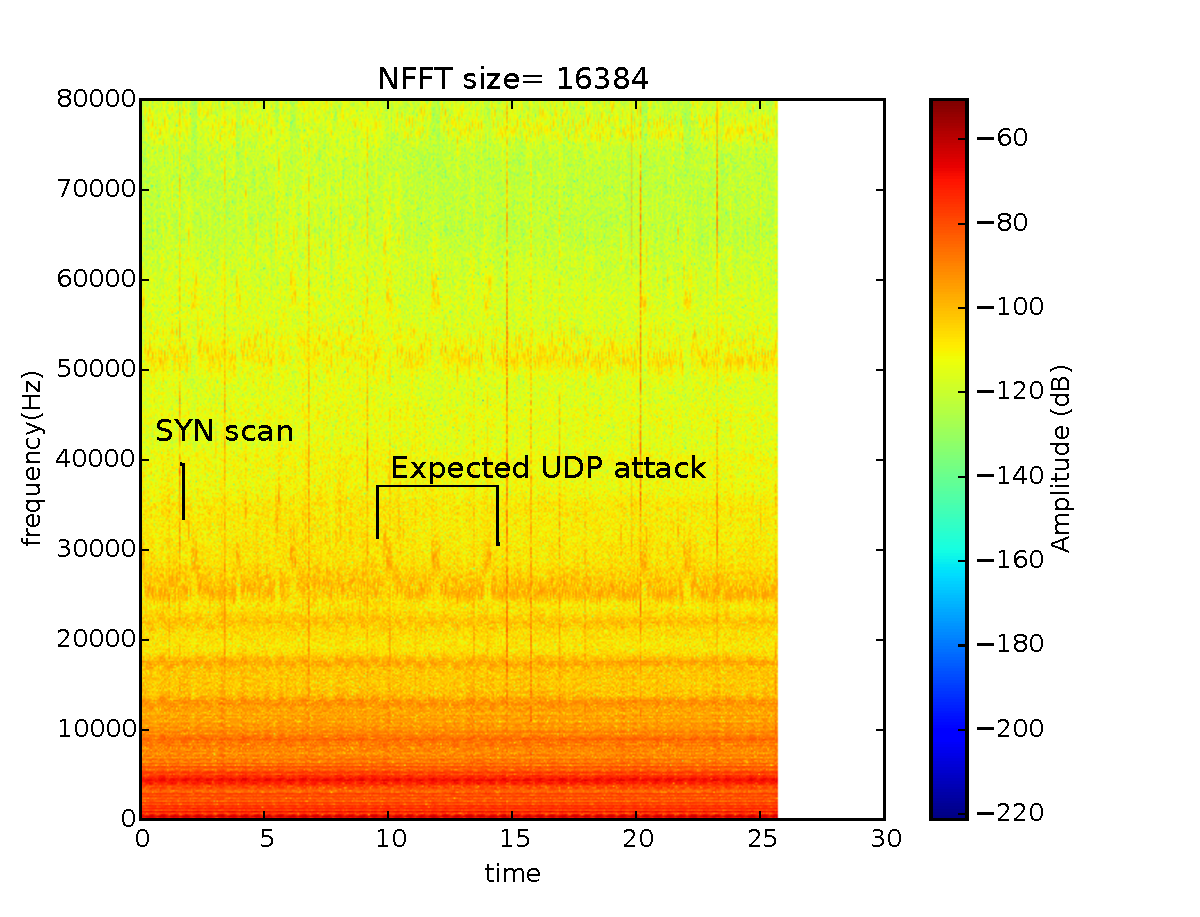
\includegraphics[width=\textwidth]{laptop_mirai_exec7_1e6_m_16384.pdf}
\caption{Mirai noise profile on Lenovo laptop. Sampling rate$=1e6$, $N=2^14$, Resolution (fs/N)=61.035 Hz}
\label{fig:laptop_mirai}
\end{figure}

Figure~\ref{fig:laptop_mirai} shows EMI generated by EMI on Lenovo laptop. As described previously, the spectrogram is annotated with the initial SYN packet spew by the bot and the attack activated for 5 minutes. Unfortunately, it does not show a continuous increase in the frequency when UDP flood attack is conducted as expected by our previous experiments. I see the increase in the frequency when I run the bot in \textbf{DEBUG} mode, which is basically the same code, but without any \textbf{fork} system calls, hence a single process.
\subsection{Spectrogram of Raspberry Pi}
Experiments conducted by running Mirai bot on Raspberry Pi.
\begin{figure}[h]
\centering
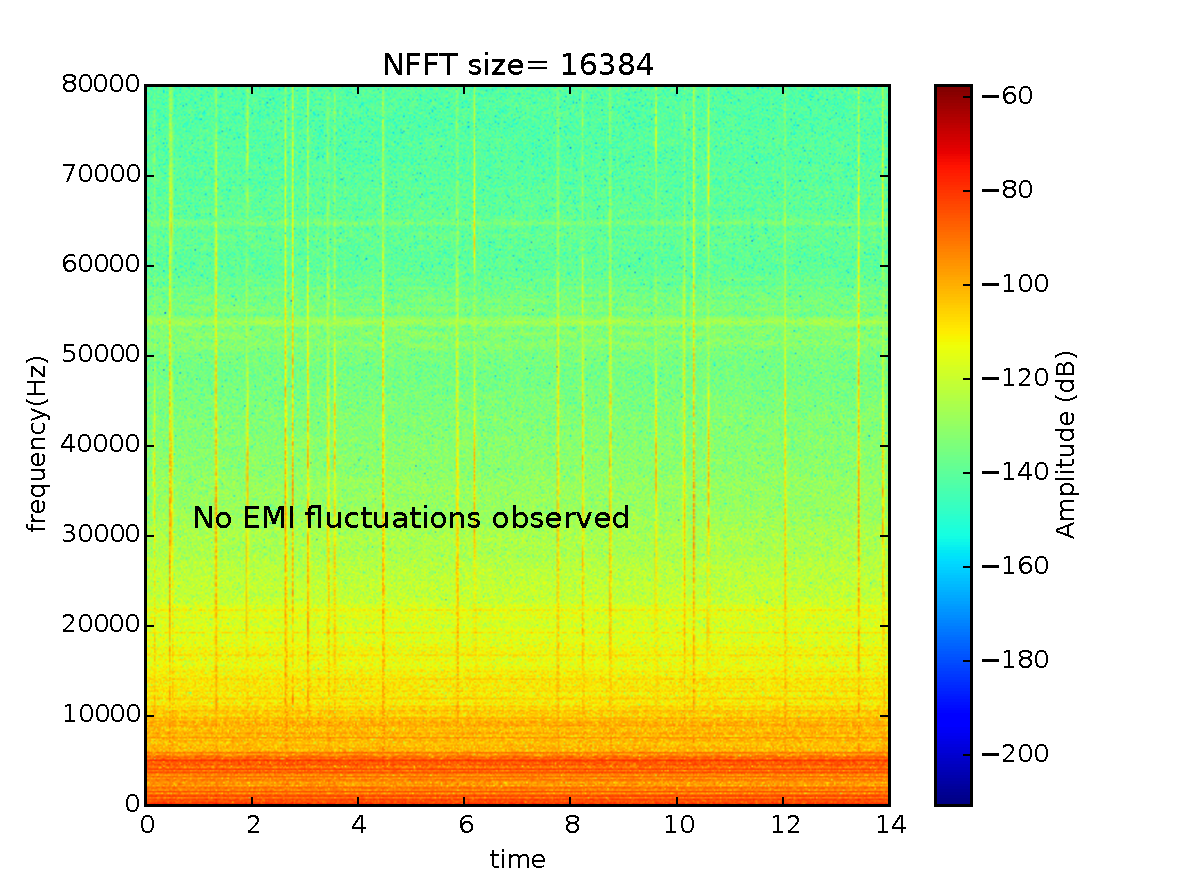
\includegraphics[width=\textwidth]{exec_2_m_16384.pdf}
\caption{Mirai noise profile on Raspberry Pi. Sampling rate$=1e6$, $N=2^14$, Resolution (fs/N)=61.035 Hz}
\label{fig:raspi_mirai}
\end{figure}

\subsection{Raspberry Pi}
I did the experiments with Raspberry Pi as the client. As with
previous experiments of UDP blasts and computation, I was not able to
see change in EMI. There are possibly two reasons for it.
\begin{itemize}
\item It uses the USB power-supply~\ref{fig:usb-raspi}. I am not clear
  about how the conversion of power supply takes place.  
\item The change in power consumed by Raspberry Pi might not be
  significant. I don't think this should be the case. A busy loop
  should have changed the noise profile in our previous experiments
  and also showed some change in noise on power-line when Mirai was
  executed.
\end{itemize}

\section{Attack from CNC}
The \ref{fig:mirai_cnc_server} shows the CNC server Mirai interface
over localhost. One attack was conducted -- UDP flood attack for 5
seconds.
\begin{figure}[t!]
%\centering
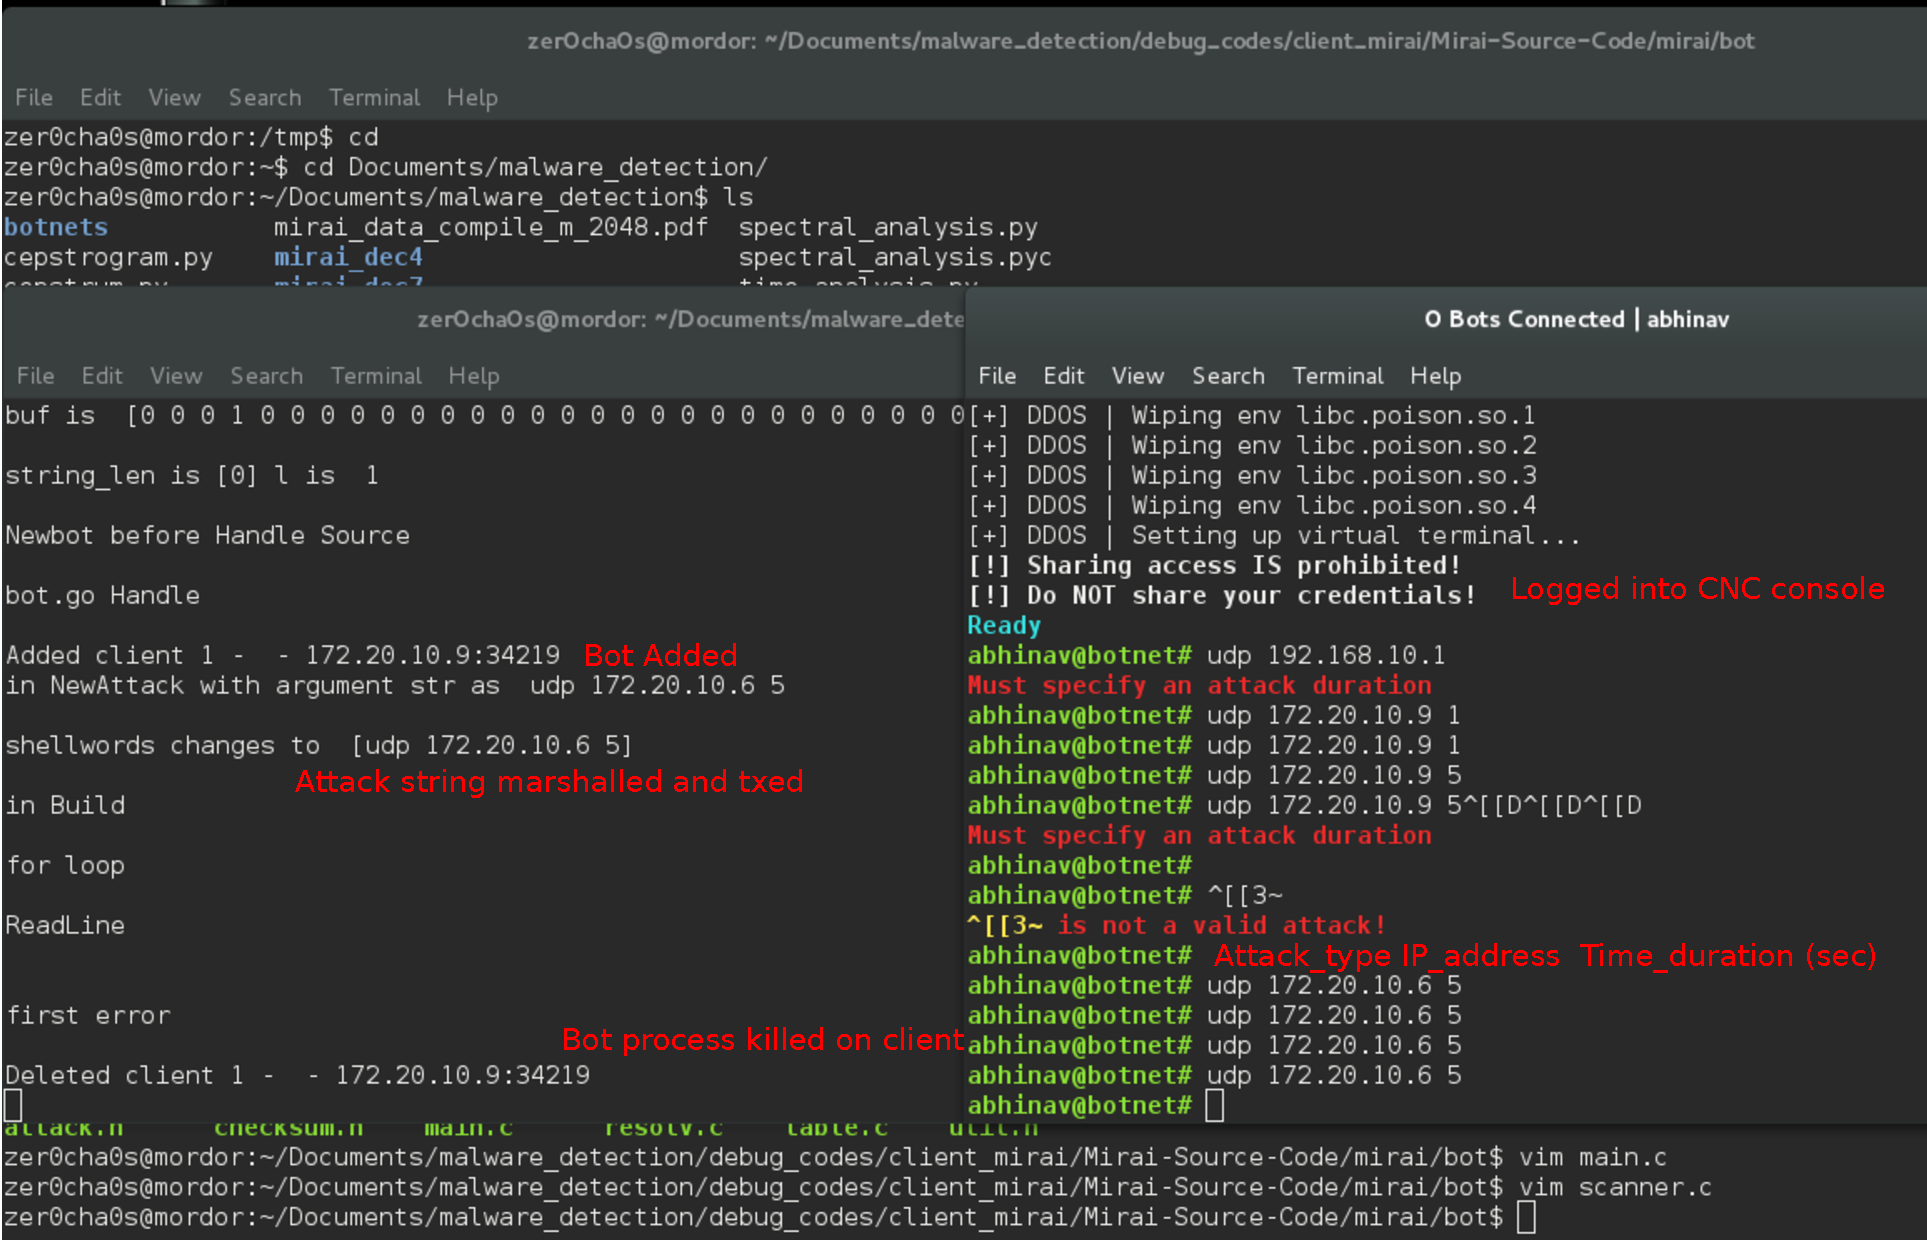
\includegraphics[width=1.3\textwidth]{mirai_attack_cnc_side.pdf}
\caption{Attack issued on CNC window. UDP flood for 5 seconds}
\label{fig:mirai_cnc_server}
\end{figure}

\begin{figure}[t!]
\centering
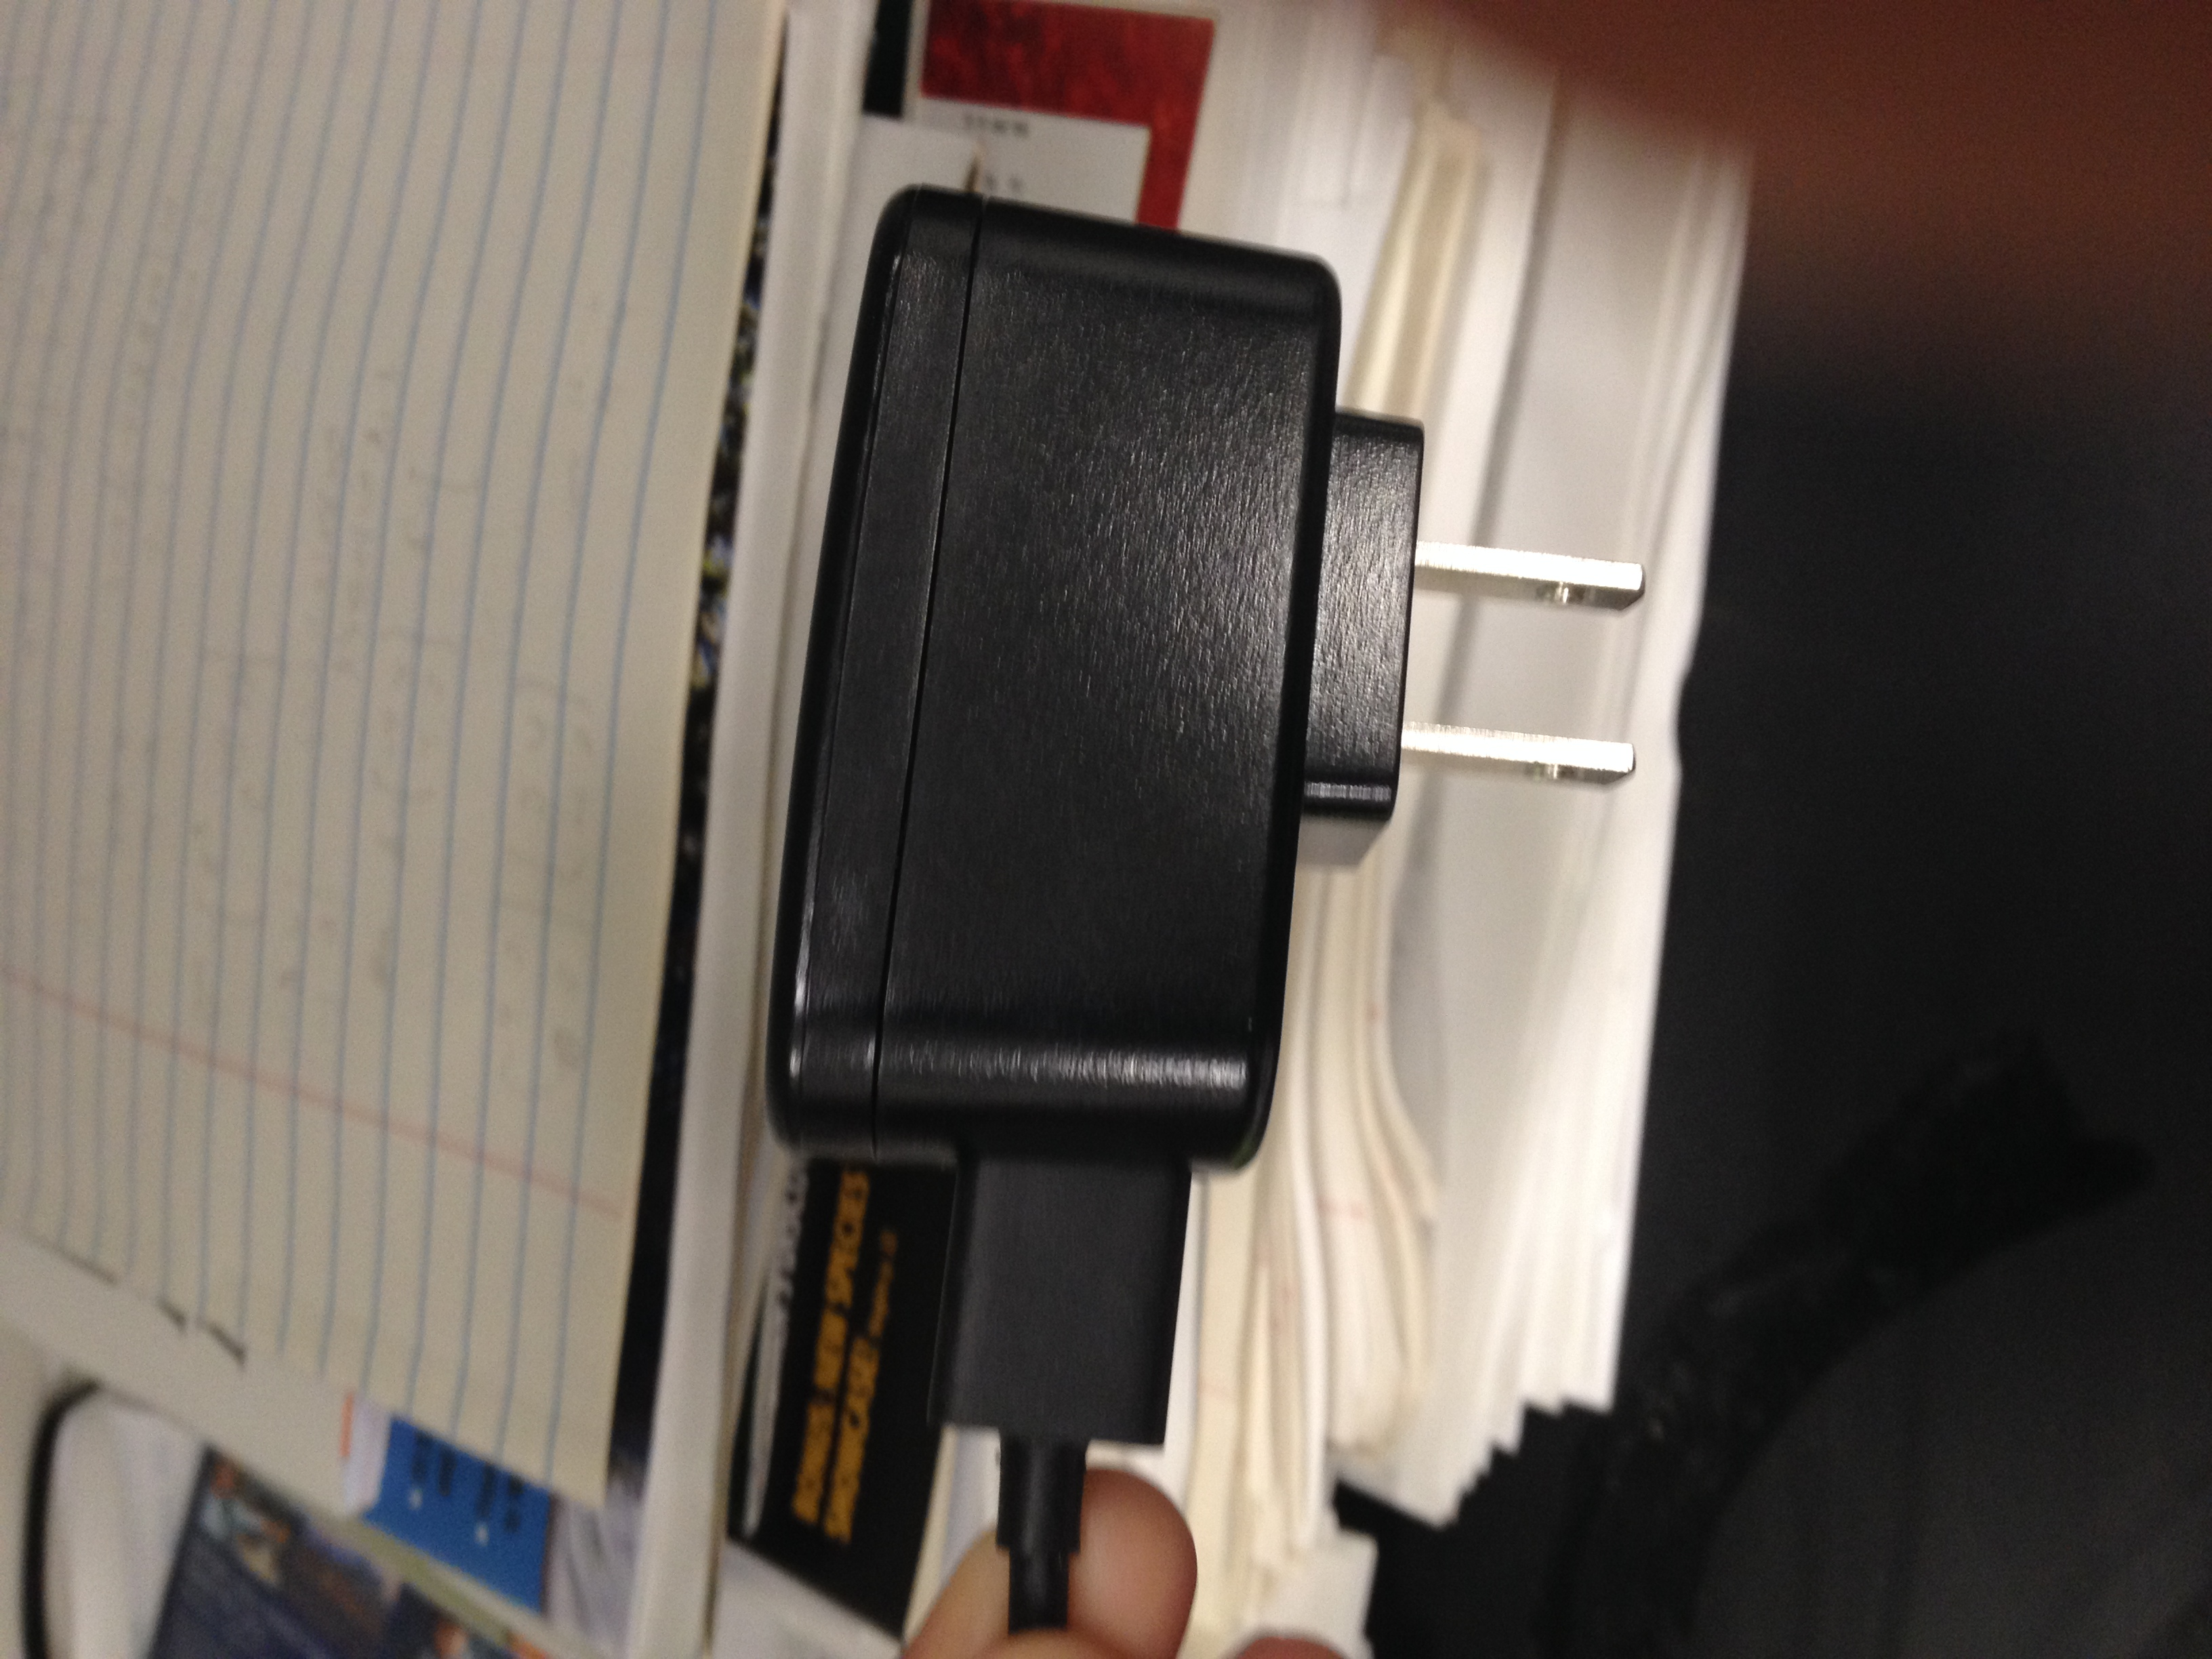
\includegraphics[width=.5\textwidth]{photo.JPG}
\caption{USB to power-line converter adapter for Raspberry Pi}
\label{fig:usb-raspi}
\end{figure}

\begin{figure}[t!]
\centering
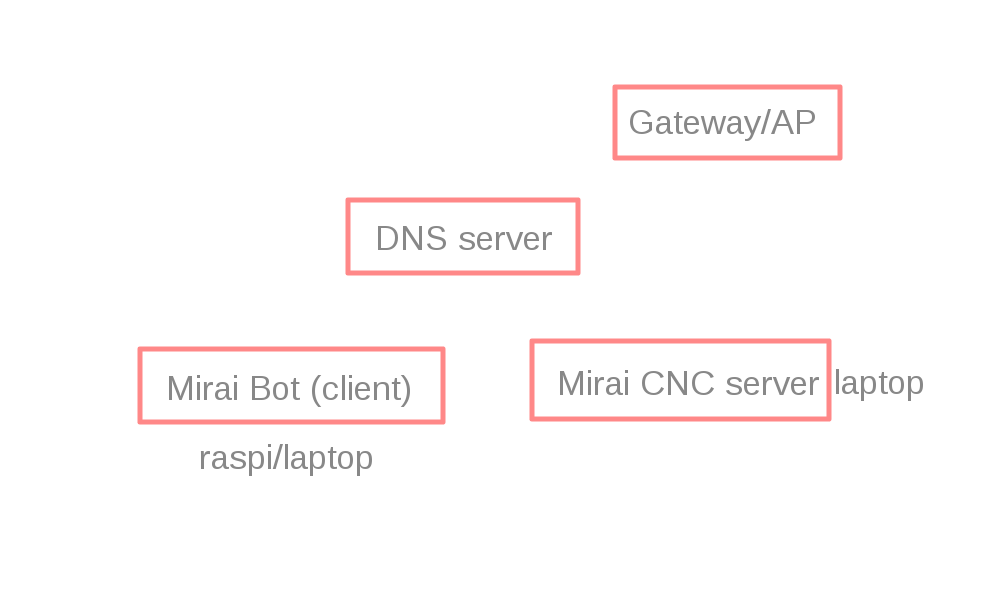
\includegraphics[width=\textwidth]{export.png}
\caption{Lab testbed on Wireless Network for the devices used. Mirai
  Bot(client) is connected to the isolated Transformer for capturing
  Power-line traces.}
\label{fig:setup}
\end{figure}


\end{document}




